\documentclass[10pt,ignorenonframetext,compress, aspectratio=169]{beamer}
\setbeamertemplate{caption}[numbered]
\setbeamertemplate{caption label separator}{: }
\setbeamercolor{caption name}{fg=normal text.fg}
\beamertemplatenavigationsymbolsempty
\usepackage{lmodern}
\usepackage{amssymb,amsmath,mathtools}
\usepackage{ifxetex,ifluatex}
\usepackage{fixltx2e} % provides \textsubscript
\ifnum 0\ifxetex 1\fi\ifluatex 1\fi=0 % if pdftex
  \usepackage[T1]{fontenc}
  \usepackage[utf8]{inputenc}
\else % if luatex or xelatex
  \ifxetex
    \usepackage{mathspec}
  \else
    \usepackage{fontspec}
  \fi
  %%\defaultfontfeatures{Ligatures=TeX,Scale=MatchLowercase}
  \defaultfontfeatures{Scale=MatchLowercase}
\fi
\usetheme[]{metropolis}
% use upquote if available, for straight quotes in verbatim environments
\IfFileExists{upquote.sty}{\usepackage{upquote}}{}
% use microtype if available
\IfFileExists{microtype.sty}{%
\usepackage{microtype}
\UseMicrotypeSet[protrusion]{basicmath} % disable protrusion for tt fonts
}{}
\newif\ifbibliography
\usepackage{color}
\usepackage{fancyvrb}
\newcommand{\VerbBar}{|}
\newcommand{\VERB}{\Verb[commandchars=\\\{\}]}
\DefineVerbatimEnvironment{Highlighting}{Verbatim}{commandchars=\\\{\}}
% Add ',fontsize=\small' for more characters per line
\usepackage{framed}
\definecolor{shadecolor}{RGB}{248,248,248}
\newenvironment{Shaded}{\begin{snugshade}}{\end{snugshade}}
\newcommand{\KeywordTok}[1]{\textcolor[rgb]{0.13,0.29,0.53}{\textbf{{#1}}}}
\newcommand{\DataTypeTok}[1]{\textcolor[rgb]{0.13,0.29,0.53}{{#1}}}
\newcommand{\DecValTok}[1]{\textcolor[rgb]{0.00,0.00,0.81}{{#1}}}
\newcommand{\BaseNTok}[1]{\textcolor[rgb]{0.00,0.00,0.81}{{#1}}}
\newcommand{\FloatTok}[1]{\textcolor[rgb]{0.00,0.00,0.81}{{#1}}}
\newcommand{\ConstantTok}[1]{\textcolor[rgb]{0.00,0.00,0.00}{{#1}}}
\newcommand{\CharTok}[1]{\textcolor[rgb]{0.31,0.60,0.02}{{#1}}}
\newcommand{\SpecialCharTok}[1]{\textcolor[rgb]{0.00,0.00,0.00}{{#1}}}
\newcommand{\StringTok}[1]{\textcolor[rgb]{0.31,0.60,0.02}{{#1}}}
\newcommand{\VerbatimStringTok}[1]{\textcolor[rgb]{0.31,0.60,0.02}{{#1}}}
\newcommand{\SpecialStringTok}[1]{\textcolor[rgb]{0.31,0.60,0.02}{{#1}}}
\newcommand{\ImportTok}[1]{{#1}}
\newcommand{\CommentTok}[1]{\textcolor[rgb]{0.56,0.35,0.01}{\textit{{#1}}}}
\newcommand{\DocumentationTok}[1]{\textcolor[rgb]{0.56,0.35,0.01}{\textbf{\textit{{#1}}}}}
\newcommand{\AnnotationTok}[1]{\textcolor[rgb]{0.56,0.35,0.01}{\textbf{\textit{{#1}}}}}
\newcommand{\CommentVarTok}[1]{\textcolor[rgb]{0.56,0.35,0.01}{\textbf{\textit{{#1}}}}}
\newcommand{\OtherTok}[1]{\textcolor[rgb]{0.56,0.35,0.01}{{#1}}}
\newcommand{\FunctionTok}[1]{\textcolor[rgb]{0.00,0.00,0.00}{{#1}}}
\newcommand{\VariableTok}[1]{\textcolor[rgb]{0.00,0.00,0.00}{{#1}}}
\newcommand{\ControlFlowTok}[1]{\textcolor[rgb]{0.13,0.29,0.53}{\textbf{{#1}}}}
\newcommand{\OperatorTok}[1]{\textcolor[rgb]{0.81,0.36,0.00}{\textbf{{#1}}}}
\newcommand{\BuiltInTok}[1]{{#1}}
\newcommand{\ExtensionTok}[1]{{#1}}
\newcommand{\PreprocessorTok}[1]{\textcolor[rgb]{0.56,0.35,0.01}{\textit{{#1}}}}
\newcommand{\AttributeTok}[1]{\textcolor[rgb]{0.77,0.63,0.00}{{#1}}}
\newcommand{\RegionMarkerTok}[1]{{#1}}
\newcommand{\InformationTok}[1]{\textcolor[rgb]{0.56,0.35,0.01}{\textbf{\textit{{#1}}}}}
\newcommand{\WarningTok}[1]{\textcolor[rgb]{0.56,0.35,0.01}{\textbf{\textit{{#1}}}}}
\newcommand{\AlertTok}[1]{\textcolor[rgb]{0.94,0.16,0.16}{{#1}}}
\newcommand{\ErrorTok}[1]{\textcolor[rgb]{0.64,0.00,0.00}{\textbf{{#1}}}}
\newcommand{\NormalTok}[1]{{#1}}
\usepackage{graphicx,grffile}
\makeatletter
\def\maxwidth{\ifdim\Gin@nat@width>\linewidth\linewidth\else\Gin@nat@width\fi}
\def\maxheight{\ifdim\Gin@nat@height>\textheight0.8\textheight\else\Gin@nat@height\fi}
\makeatother
% Scale images if necessary, so that they will not overflow the page
% margins by default, and it is still possible to overwrite the defaults
% using explicit options in \includegraphics[width, height, ...]{}
\setkeys{Gin}{width=\maxwidth,height=\maxheight,keepaspectratio}

% Prevent slide breaks in the middle of a paragraph:
\widowpenalties 1 10000
\raggedbottom

\AtBeginPart{
  \let\insertpartnumber\relax
  \let\partname\relax
  \frame{\partpage}
}
\AtBeginSection{
  \ifbibliography
  \else
    \let\insertsectionnumber\relax
    \let\sectionname\relax
    \frame{\sectionpage}
  \fi
}
\AtBeginSubsection{
  \let\insertsubsectionnumber\relax
  \let\subsectionname\relax
  \frame{\subsectionpage}
}

\setlength{\parindent}{0pt}
\setlength{\parskip}{6pt plus 2pt minus 1pt}
\setlength{\emergencystretch}{3em}  % prevent overfull lines
\providecommand{\tightlist}{%
  \setlength{\itemsep}{0pt}\setlength{\parskip}{0pt}}
\setcounter{secnumdepth}{0}

%% GLS Added
% Textcomp for various common symbols
\usepackage{textcomp}

\usepackage{booktabs}

% Creative Commons Icons
\usepackage[scale=1]{ccicons}

\newenvironment{centrefig}{\begin{figure}\centering}{\end{figure}}
\newcommand{\columnsbegin}{\begin{columns}}
\newcommand{\columnsend}{\end{columns}}
\newcommand{\centreFigBegin}{\begin{figure}\centering}
\newcommand{\centreFigEnd}{\end{figure}}
%%

\DefineVerbatimEnvironment{Highlighting}{Verbatim}{commandchars=\\\{\}, fontsize=\tiny}
% make console-output smaller:
\makeatletter
\def\verbatim{\tiny\@verbatim \frenchspacing\@vobeyspaces \@xverbatim}
\makeatother
\setlength{\parskip}{0pt}
\setlength{\OuterFrameSep}{-4pt} % was -4pt
\makeatletter
\preto{\@verbatim}{\topsep=-10pt \partopsep=-10pt} % were -10pt
\makeatother

\title{Generalized Additive Models}
\author{Gavin L. Simpson}
\date{February, 2017}

\begin{document}
\frame{\titlepage}

\section{Generalized additive models}\label{generalized-additive-models}

\begin{frame}{Generalized additive models}

\alert{Generalized additive models}

\begin{itemize}
\tightlist
\item
  Generalized --- conditions distribution of \(y\) from (extended)
  exponential family of distributions
\item
  Additive --- assume nothing more that separate model component sum
\item
  Models --- it's a model
\end{itemize}

Earlier we looked at models that look like

\[
y_i = \beta_0 + \beta_1 x_{1i} + \beta_2 x_{2i} + \cdots + \varepsilon_i
\]

\(\hat{y}_i\) is a linear combination of covariates

GLMs extend this model to allow \(y_i\) to be distributed any member of
the exponential family

Conditional distribution of \(y_i | \mathbf{X}\)

\end{frame}

\begin{frame}{Is this linear?}

\begin{center}\includegraphics[width=0.7\linewidth]{02-gams_files/figure-beamer/islinear-1} \end{center}

\end{frame}

\begin{frame}[fragile]{Is this linear? Maybe?}

\begin{Shaded}
\begin{Highlighting}[]
\NormalTok{>}\StringTok{ }\KeywordTok{lm}\NormalTok{(y ~}\StringTok{ }\NormalTok{x1, }\DataTypeTok{data=}\NormalTok{dat)}
\end{Highlighting}
\end{Shaded}

\begin{Shaded}
\begin{Highlighting}[]
\NormalTok{>}\StringTok{ }\KeywordTok{ggplot}\NormalTok{(dat, }\KeywordTok{aes}\NormalTok{(}\DataTypeTok{y=}\NormalTok{y, }\DataTypeTok{x=}\NormalTok{x1)) +}\StringTok{ }\KeywordTok{geom_point}\NormalTok{() +}
\NormalTok{+}\StringTok{     }\KeywordTok{geom_smooth}\NormalTok{(}\DataTypeTok{method=}\StringTok{"lm"}\NormalTok{)}
\end{Highlighting}
\end{Shaded}

\begin{center}\includegraphics[width=0.7\linewidth]{02-gams_files/figure-beamer/maybe-1} \end{center}

\end{frame}

\begin{frame}[fragile]{What can we do?}

\begin{Shaded}
\begin{Highlighting}[]
\NormalTok{>}\StringTok{ }\KeywordTok{lm}\NormalTok{(y ~}\StringTok{ }\NormalTok{x1 +}\StringTok{ }\KeywordTok{poly}\NormalTok{(x1, }\DecValTok{2}\NormalTok{), }\DataTypeTok{data=}\NormalTok{dat)}
\end{Highlighting}
\end{Shaded}

\begin{Shaded}
\begin{Highlighting}[]
\NormalTok{>}\StringTok{ }\KeywordTok{ggplot}\NormalTok{(dat, }\KeywordTok{aes}\NormalTok{(}\DataTypeTok{y=}\NormalTok{y, }\DataTypeTok{x=}\NormalTok{x1)) +}\StringTok{ }\KeywordTok{geom_point}\NormalTok{() +}
\NormalTok{+}\StringTok{     }\KeywordTok{geom_smooth}\NormalTok{(}\DataTypeTok{method=}\StringTok{"lm"}\NormalTok{, }\DataTypeTok{formula =} \NormalTok{y~}\KeywordTok{poly}\NormalTok{(x, }\DecValTok{2}\NormalTok{))}
\end{Highlighting}
\end{Shaded}

\begin{center}\includegraphics[width=0.7\linewidth]{02-gams_files/figure-beamer/quadratic-1} \end{center}

\end{frame}

\begin{frame}[fragile]{How practical is this?}

\begin{itemize}
\tightlist
\item
  Adding in quadratic (and higher terms) \emph{can} make sense
\item
  This feels a bit \emph{ad hoc}
\item
  Better if we had a \textbf{framework} to deal with these issues?
\end{itemize}

\begin{Shaded}
\begin{Highlighting}[]
\NormalTok{>}\StringTok{ }\KeywordTok{ggplot}\NormalTok{(dat, }\KeywordTok{aes}\NormalTok{(}\DataTypeTok{y=}\NormalTok{y, }\DataTypeTok{x=}\NormalTok{x2)) +}\StringTok{ }\KeywordTok{geom_point}\NormalTok{() +}
\NormalTok{+}\StringTok{     }\KeywordTok{geom_smooth}\NormalTok{(}\DataTypeTok{method=}\StringTok{"lm"}\NormalTok{, }\DataTypeTok{formula =} \NormalTok{y~}\KeywordTok{poly}\NormalTok{(x, }\DecValTok{2}\NormalTok{))}
\end{Highlighting}
\end{Shaded}

\begin{center}\includegraphics[width=0.7\linewidth]{02-gams_files/figure-beamer/ruhroh-1} \end{center}

\end{frame}

\begin{frame}{What does a GAM look like?}

\[
y_i = \beta_0 + \sum_j s_j(x_{ji}) + \varepsilon_i
\]

where \(\epsilon_i \sim N(0, \sigma^2)\), \(y_i \sim \text{Normal}\)
(for now)

Remember that we're modelling the mean of this distribution!

Call the above equation the \textbf{linear predictor}

\end{frame}

\begin{frame}[fragile]{What are these \(s_j\)?}

\columnsbegin

\column{0.5\linewidth}

\begin{itemize}
\tightlist
\item
  Think \(s\) = \textbf{smooth}
\item
  Want to model the covariates flexibly
\item
  Covariates and response not necessarily linearly related!
\item
  Want some ``wiggles''
\end{itemize}

\column{0.5\linewidth}

\begin{Shaded}
\begin{Highlighting}[]
\NormalTok{>}\StringTok{ }\NormalTok{spdat <-}\StringTok{ }\KeywordTok{melt}\NormalTok{(dat, }\DataTypeTok{id.vars =} \KeywordTok{c}\NormalTok{(}\StringTok{"y"}\NormalTok{))}
\NormalTok{>}\StringTok{ }\NormalTok{p <-}\StringTok{ }\KeywordTok{ggplot}\NormalTok{(spdat,}\KeywordTok{aes}\NormalTok{(}\DataTypeTok{y=}\NormalTok{y,}\DataTypeTok{x=}\NormalTok{value)) +}
\NormalTok{+}\StringTok{       }\KeywordTok{geom_point}\NormalTok{() +}
\NormalTok{+}\StringTok{       }\KeywordTok{facet_wrap}\NormalTok{(~variable, }\DataTypeTok{nrow=}\DecValTok{2}\NormalTok{)}
\NormalTok{>}\StringTok{ }\KeywordTok{print}\NormalTok{(p)}
\end{Highlighting}
\end{Shaded}

\begin{center}\includegraphics[width=0.7\linewidth]{02-gams_files/figure-beamer/smoothdat-1} \end{center}

\columnsend

\end{frame}

\begin{frame}[fragile]{What are these \(s_j\)?}

\columnsbegin

\column{0.5\linewidth}

\begin{itemize}
\tightlist
\item
  Think \(s\) = \textbf{smooth}
\item
  Want to model the covariates flexibly
\item
  Covariates and response not necessarily linearly related!
\item
  Want some ``wiggles''
\end{itemize}

\column{0.5\linewidth}

\begin{Shaded}
\begin{Highlighting}[]
\NormalTok{>}\StringTok{ }\NormalTok{p <-}\StringTok{ }\NormalTok{p +}\StringTok{ }\KeywordTok{geom_smooth}\NormalTok{()}
\NormalTok{>}\StringTok{ }\KeywordTok{print}\NormalTok{(p)}
\end{Highlighting}
\end{Shaded}

\begin{center}\includegraphics[width=0.7\linewidth]{02-gams_files/figure-beamer/wsmooths-1} \end{center}

\columnsend

\end{frame}

\begin{frame}{Straight lines vs.~interpolation}

\columnsbegin
\column{0.55\linewidth}

\begin{itemize}
\tightlist
\item
  Want a line that is ``close'' to all the data
\item
  Don't want interpolation -- we know there is ``error''
\item
  Balance between interpolation and ``fit''
\end{itemize}

\column{0.45\linewidth}

\begin{center}\includegraphics[width=0.7\linewidth]{02-gams_files/figure-beamer/wiggles-1} \end{center}

\columnsend

\end{frame}

\begin{frame}{Splines}

\begin{itemize}
\tightlist
\item
  Functions made of other, simpler functions
\item
  \textbf{Basis functions} \(b_k\), estimate \(\beta_k\)
\item
  \(s(x) = \sum_{k=1}^K \beta_k b_k(x)\)
\item
  Makes the math(s) much easier
\end{itemize}

\begin{center}\includegraphics[width=\linewidth]{02-gams_files/figure-beamer/erics-spline-figure-1} \end{center}

\end{frame}

\begin{frame}{Design matrices}

We often write models as \(X\boldsymbol{\beta}\)

\begin{itemize}
\tightlist
\item
  \(X\) is our data
\item
  \(\boldsymbol{\beta}\) are parameters we need to estimate
\end{itemize}

For a GAM it's the same

\begin{itemize}
\tightlist
\item
  \(X\) has columns for each basis, evaluated at each observation
\item
  again, this is the linear predictor
\end{itemize}

\end{frame}

\begin{frame}{Measuring wigglyness}

Visually:

\begin{itemize}
\tightlist
\item
  Lots of wiggles == NOT SMOOTH
\item
  Straight line == VERY SMOOTH
\end{itemize}

How do we do this mathematically?

\begin{itemize}
\tightlist
\item
  Derivatives!
\item
  (Calculus \emph{was} a useful class after all!)
\end{itemize}

\end{frame}

\begin{frame}{Wiggliness by derivatives}

\begin{figure}[htbp]
\centering
\includegraphics{wiggly.gif}
\caption{Animation of derivatives}
\end{figure}

\end{frame}

\begin{frame}{What was that grey bit?}

\[
\int_\mathbb{R} \left( \frac{\partial^2 f(x)}{\partial^2 x}\right)^2 \text{d}x
\]

Take some derivatives of the smooth and integrate them over \(x\)

\emph{Turns out} we can always write this as
\(\boldsymbol{\beta}^{\text{T}}S\boldsymbol{\beta}\), so the
\(\boldsymbol{\beta}\) is separate from the derivatives

Call \(S\) the \textbf{penalty matrix}

\end{frame}

\begin{frame}{Making wigglyness matter}

\begin{itemize}
\tightlist
\item
  \(\boldsymbol{\beta}^\text{T}S\boldsymbol{\beta}\) measures wigglyness
\item
  ``Likelihood'' measures closeness to the data
\item
  Penalize closeness to the data\ldots{}
\item
  Use a \textbf{smoothing parameter} to decide on that trade-off\ldots{}
\item
  \(\lambda \beta^\text{T}S\beta\)
\item
  Estimate the \(\beta_k\) terms but penalise objective
\item
  ``closeness to data'' + penalty
\end{itemize}

\end{frame}

\begin{frame}{Smoothing parameter}

\begin{center}\includegraphics[width=0.95\linewidth]{02-gams_files/figure-beamer/wiggles-plot-1} \end{center}

\end{frame}

\begin{frame}{Smoothing parameter selection}

\begin{itemize}
\tightlist
\item
  Many methods: AIC, Mallow's \(C_p\), GCV, ML, REML
\item
  Recommendation, based on simulation and practice:

  \begin{itemize}
  \tightlist
  \item
    Use REML or ML
  \item
    Reiss \& Ogden (2009), Wood (2011)
  \end{itemize}
\end{itemize}

\begin{figure}[htbp]
\centering
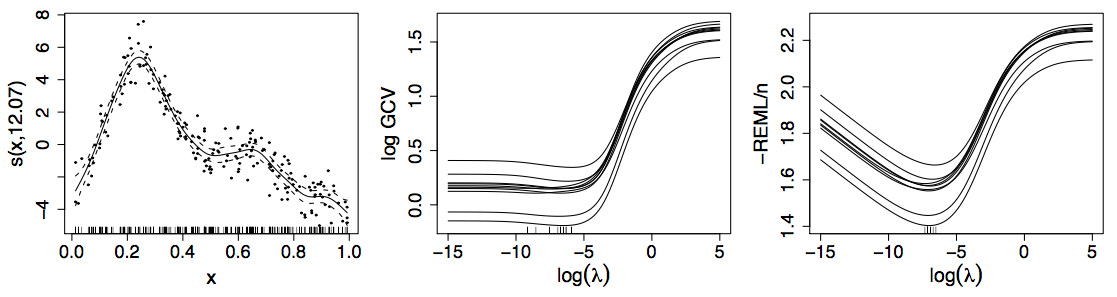
\includegraphics{remlgcv.png}
\caption{REML smoothness selection}
\end{figure}

\end{frame}

\begin{frame}{Maximum wiggliness}

\begin{itemize}
\tightlist
\item
  We can set \textbf{basis complexity} or ``size'' (\(k\))

  \begin{itemize}
  \tightlist
  \item
    Maximum wigglyness
  \end{itemize}
\item
  Smooths have \textbf{effective degrees of freedom} (EDF)
\item
  EDF \textless{} \(k\)
\item
  Set \(k\) ``large enough''

  \begin{itemize}
  \tightlist
  \item
    Penalty does the rest
  \end{itemize}
\end{itemize}

More on this in a bit\ldots{}

\end{frame}

\begin{frame}{GAM summary}

\begin{itemize}
\tightlist
\item
  Straight lines suck --- the world is not linear --- we want
  \textbf{wiggles}
\item
  Use little functions (\textbf{basis functions}) to make big functions
  (\textbf{smooths})
\item
  Need to make sure your smooths are \textbf{wiggly enough}
\item
  Use a \textbf{penalty} to trade off wiggliness/generality
\end{itemize}

\end{frame}

\section{Fitting GAMs in practice}\label{fitting-gams-in-practice}

\begin{frame}[fragile]{Translating maths into R}

A simple example:

\[
y_i = \beta_0 + s(x) + s(w) + \epsilon_i
\]

where \(\epsilon_i \sim N(0, \sigma^2)\)

Let's pretend that \(y_i \sim \text{Normal}\)

\begin{itemize}
\tightlist
\item
  linear predictor:
  \texttt{formula\ =\ y\ \textasciitilde{}\ s(x)\ +\ s(w)}
\item
  response distribution: \texttt{family\ =\ gaussian()}
\item
  data: \texttt{data=some\_data\_frame}
\end{itemize}

\texttt{method="REML"} uses REML for smoothness selection (default is
\texttt{"GCV.Cp"})

\begin{Shaded}
\begin{Highlighting}[]
\NormalTok{>}\StringTok{ }\NormalTok{my_model <-}\StringTok{ }\KeywordTok{gam}\NormalTok{(y ~}\StringTok{ }\KeywordTok{s}\NormalTok{(x) +}\StringTok{ }\KeywordTok{s}\NormalTok{(w),}
\NormalTok{+}\StringTok{                 }\DataTypeTok{family =} \KeywordTok{gaussian}\NormalTok{(), }\DataTypeTok{data =} \NormalTok{some_data_frame,}
\NormalTok{+}\StringTok{                 }\DataTypeTok{method =} \StringTok{"REML"}\NormalTok{)}
\end{Highlighting}
\end{Shaded}

\end{frame}

\section{Checking the basis size}\label{checking-the-basis-size}

\begin{frame}{How well does the model fit?}

\begin{itemize}
\tightlist
\item
  Many choices: k, family, type of smoother, \ldots{}
\item
  How do we assess how well our model fits?
\end{itemize}

\end{frame}

\begin{frame}[fragile]{Example functions}

\begin{Shaded}
\begin{Highlighting}[]
\NormalTok{>}\StringTok{ }\KeywordTok{set.seed}\NormalTok{(}\DecValTok{2}\NormalTok{)}
\NormalTok{>}\StringTok{ }\NormalTok{n <-}\StringTok{  }\DecValTok{400}
\NormalTok{>}\StringTok{ }\NormalTok{x1 <-}\StringTok{  }\KeywordTok{rnorm}\NormalTok{(n)}
\NormalTok{>}\StringTok{ }\NormalTok{x2 <-}\StringTok{ }\KeywordTok{rnorm}\NormalTok{(n)}
\NormalTok{>}\StringTok{ }\NormalTok{y_val <-}\StringTok{ }\DecValTok{1} \NormalTok{+}\StringTok{ }\DecValTok{2} \NormalTok{*}\StringTok{ }\KeywordTok{cos}\NormalTok{(pi *}\StringTok{ }\NormalTok{x1) +}\StringTok{ }\DecValTok{2} \NormalTok{/}\StringTok{ }\NormalTok{(}\DecValTok{1} \NormalTok{+}\StringTok{ }\KeywordTok{exp}\NormalTok{(-}\DecValTok{5} \NormalTok{*}\StringTok{ }\NormalTok{(x2)))}
\NormalTok{>}\StringTok{ }\NormalTok{y_norm <-}\StringTok{ }\NormalTok{y_val +}\StringTok{ }\KeywordTok{rnorm}\NormalTok{(n, }\DecValTok{0}\NormalTok{, }\FloatTok{0.5}\NormalTok{)}
\end{Highlighting}
\end{Shaded}

\begin{Shaded}
\begin{Highlighting}[]
\NormalTok{>}\StringTok{ }\KeywordTok{layout}\NormalTok{(}\KeywordTok{matrix}\NormalTok{(}\DecValTok{1}\NormalTok{:}\DecValTok{2}\NormalTok{, }\DataTypeTok{ncol=}\DecValTok{2}\NormalTok{))}
\NormalTok{>}\StringTok{ }\KeywordTok{plot}\NormalTok{(x1,y_norm); }\KeywordTok{plot}\NormalTok{(x2,y_norm)}
\NormalTok{>}\StringTok{ }\KeywordTok{layout}\NormalTok{(}\DecValTok{1}\NormalTok{)}
\end{Highlighting}
\end{Shaded}

\begin{center}\includegraphics[width=0.8\linewidth]{02-gams_files/figure-beamer/sims_plot-1} \end{center}

\end{frame}

\begin{frame}[fragile]{Basis size (k)}

\begin{itemize}
\tightlist
\item
  Set \texttt{k} per term
\item
  e.g. \texttt{s(x,\ k=10)} or \texttt{s(x,\ y,\ k=100)}
\item
  Penalty removes ``extra'' wigglyness

  \begin{itemize}
  \tightlist
  \item
    \emph{up to a point!}
  \end{itemize}
\item
  But computation is slower with bigger \texttt{k}
\end{itemize}

\end{frame}

\begin{frame}[fragile]{Checking basis size --- \texttt{gam.check()}}

\begin{Shaded}
\begin{Highlighting}[]
\NormalTok{>}\StringTok{ }\NormalTok{norm_model_1 <-}\StringTok{ }\KeywordTok{gam}\NormalTok{(y_norm ~}\StringTok{ }\KeywordTok{s}\NormalTok{(x1,}\DataTypeTok{k=}\DecValTok{4}\NormalTok{) +}\StringTok{ }\KeywordTok{s}\NormalTok{(x2,}\DataTypeTok{k=}\DecValTok{4}\NormalTok{), }\DataTypeTok{method =} \StringTok{"REML"}\NormalTok{)}
\NormalTok{>}\StringTok{ }\KeywordTok{gam.check}\NormalTok{(norm_model_1)}
\end{Highlighting}
\end{Shaded}

\begin{verbatim}

Method: REML   Optimizer: outer newton
full convergence after 8 iterations.
Gradient range [-0.0003467788,0.0005154578]
(score 736.9402 & scale 2.252304).
Hessian positive definite, eigenvalue range [0.000346021,198.5041].
Model rank =  7 / 7 

Basis dimension (k) checking results. Low p-value (k-index<1) may
indicate that k is too low, especially if edf is close to k'.

         k'   edf k-index p-value
s(x1) 3.000 1.002   0.125    0.00
s(x2) 3.000 2.914   1.045    0.82
\end{verbatim}

\end{frame}

\begin{frame}[fragile]{Checking basis size --- \texttt{gam.check()}}

\begin{Shaded}
\begin{Highlighting}[]
\NormalTok{>}\StringTok{ }\NormalTok{norm_model_2 <-}\StringTok{ }\KeywordTok{gam}\NormalTok{(y_norm ~}\StringTok{ }\KeywordTok{s}\NormalTok{(x1, }\DataTypeTok{k=}\DecValTok{12}\NormalTok{) +}\StringTok{ }\KeywordTok{s}\NormalTok{(x2, }\DataTypeTok{k=}\DecValTok{4}\NormalTok{), }\DataTypeTok{method =} \StringTok{"REML"}\NormalTok{)}
\NormalTok{>}\StringTok{ }\KeywordTok{gam.check}\NormalTok{(norm_model_2)}
\end{Highlighting}
\end{Shaded}

\begin{verbatim}

Method: REML   Optimizer: outer newton
full convergence after 11 iterations.
Gradient range [-5.658609e-06,5.392657e-06]
(score 345.3111 & scale 0.2706205).
Hessian positive definite, eigenvalue range [0.967727,198.6299].
Model rank =  15 / 15 

Basis dimension (k) checking results. Low p-value (k-index<1) may
indicate that k is too low, especially if edf is close to k'.

          k'    edf k-index p-value
s(x1) 11.000 10.837   0.989    0.36
s(x2)  3.000  2.984   0.861    0.00
\end{verbatim}

\end{frame}

\begin{frame}[fragile]{Checking basis size --- \texttt{gam.check()}}

\begin{Shaded}
\begin{Highlighting}[]
\NormalTok{>}\StringTok{ }\NormalTok{norm_model_3 <-}\StringTok{ }\KeywordTok{gam}\NormalTok{(y_norm~}\KeywordTok{s}\NormalTok{(x1,}\DataTypeTok{k=}\DecValTok{12}\NormalTok{)+}\KeywordTok{s}\NormalTok{(x2,}\DataTypeTok{k=}\DecValTok{12}\NormalTok{),}\DataTypeTok{method=} \StringTok{"REML"}\NormalTok{)}
\NormalTok{>}\StringTok{ }\KeywordTok{gam.check}\NormalTok{(norm_model_3)}
\end{Highlighting}
\end{Shaded}

\begin{verbatim}

Method: REML   Optimizer: outer newton
full convergence after 8 iterations.
Gradient range [-5.103686e-05,-1.089481e-08]
(score 334.2084 & scale 0.2485446).
Hessian positive definite, eigenvalue range [2.812257,198.6868].
Model rank =  23 / 23 

Basis dimension (k) checking results. Low p-value (k-index<1) may
indicate that k is too low, especially if edf is close to k'.

          k'    edf k-index p-value
s(x1) 11.000 10.848   0.976    0.30
s(x2) 11.000  7.948   0.946    0.14
\end{verbatim}

\end{frame}

\begin{frame}[fragile]{Checking basis size --- \texttt{gam.check()}}

\begin{Shaded}
\begin{Highlighting}[]
\NormalTok{>}\StringTok{ }\KeywordTok{layout}\NormalTok{(}\KeywordTok{matrix}\NormalTok{(}\DecValTok{1}\NormalTok{:}\DecValTok{6}\NormalTok{,}\DataTypeTok{ncol=}\DecValTok{2}\NormalTok{, }\DataTypeTok{byrow =} \OtherTok{TRUE}\NormalTok{))}
\NormalTok{>}\StringTok{ }\NormalTok{op <-}\StringTok{ }\KeywordTok{par}\NormalTok{(}\DataTypeTok{mar =} \KeywordTok{c}\NormalTok{(}\DecValTok{5}\NormalTok{,}\DecValTok{4}\NormalTok{,}\DecValTok{2}\NormalTok{,}\DecValTok{2}\NormalTok{) +}\StringTok{ }\FloatTok{0.1}\NormalTok{)}
\NormalTok{>}\StringTok{ }\KeywordTok{plot}\NormalTok{(norm_model_1)}
\NormalTok{>}\StringTok{ }\KeywordTok{plot}\NormalTok{(norm_model_2)}
\NormalTok{>}\StringTok{ }\KeywordTok{plot}\NormalTok{(norm_model_3)}
\NormalTok{>}\StringTok{ }\KeywordTok{par}\NormalTok{(op)}
\NormalTok{>}\StringTok{ }\KeywordTok{layout}\NormalTok{(}\DecValTok{1}\NormalTok{)}
\end{Highlighting}
\end{Shaded}

\begin{center}\includegraphics[width=0.7\linewidth]{02-gams_files/figure-beamer/gam_check_norm4-1} \end{center}

\end{frame}

\section{Model selection}\label{model-selection}

\begin{frame}[fragile]{Overview}

\begin{itemize}
\tightlist
\item
  Model selection
\item
  Shrinkage smooths
\item
  Shrinkage via double penalty (\texttt{select\ =\ TRUE})
\item
  Confidence intervals for smooths
\item
  \emph{p} values
\item
  \texttt{anova()}
\item
  AIC
\end{itemize}

\end{frame}

\begin{frame}{Model selection}

Model (or variable) selection --- and important area of theoretical and
applied interest

\begin{itemize}
\tightlist
\item
  In statistics we aim for a balance between \emph{fit} and
  \emph{parsimony}
\item
  In applied research we seek the set of covariates with strongest
  effects on \(y\)
\end{itemize}

We seek a subset of covariates that improves \emph{interpretability} and
\emph{prediction accuracy}

\end{frame}

\section{Shrinkage \& additional
penalties}\label{shrinkage-additional-penalties}

\begin{frame}{Shrinkage \& additional penalties}

Smoothing parameter estimation allows selection of a wide range of
potentially complex functions for smooths\ldots{}

But, cannot remove a term entirely from the model because the penalties
used act only on the \emph{range space} of a spline basis. The
\emph{null space} of the basis is unpenalized.

\begin{itemize}
\tightlist
\item
  \textbf{Null space} --- the basis functions that are smooth (constant,
  linear)
\item
  \textbf{Range space} --- the basis functions that are wiggly
\end{itemize}

\end{frame}

\begin{frame}[fragile]{Shrinkage \& additional penalties}

\textbf{mgcv} has two ways to penalize the null space, i.e.~to do
selection

\begin{itemize}
\tightlist
\item
  \emph{double penalty approach} via \texttt{select\ =\ TRUE}
\item
  \emph{shrinkage approach} via special bases for thin plate and cubic
  splines
\end{itemize}

Other shrinkage/selection approaches are available

\end{frame}

\begin{frame}{Double-penalty shrinkage}

\(\mathbf{S}_j\) is the smoothing penalty matrix \& can be decomposed as

\[
\mathbf{S}_j = \mathbf{U}_j\boldsymbol{\Lambda}_j\mathbf{U}_j^{T}
\]

where \(\mathbf{U}_j\) is a matrix of eigenvectors and
\(\boldsymbol{\Lambda}_j\) a diagonal matrix of eigenvalues (i.e.~this
is an eigen decomposition of \(\mathbf{S}_j\)).

\(\boldsymbol{\Lambda}_j\) contains some \textbf{0}s due to the spline
basis null space --- no matter how large the penalty \(\lambda_j\) might
get no guarantee a smooth term will be suppressed completely.

To solve this we need an extra penalty\ldots{}

\end{frame}

\begin{frame}[fragile]{Double-penalty shrinkage}

Create a second penalty matrix from \(\mathbf{U}_j\), considering only
the matrix of eigenvectors associated with the zero eigenvalues

\[
\mathbf{S}_j^{*} = \mathbf{U}_j^{*}\mathbf{U}_j^{*T}
\]

Now we can fit a GAM with two penalties of the form

\[
\lambda_j \mathbf{\beta}^T \mathbf{S}_j \mathbf{\beta} + \lambda_j^{*} \mathbf{\beta}^T \mathbf{S}_j^{*} \mathbf{\beta}
\]

Which implies two sets of penalties need to be estimated.

In practice, add \texttt{select\ =\ TRUE} to your \texttt{gam()} call

\end{frame}

\begin{frame}[fragile]{Shrinkage}

The double penalty approach requires twice as many smoothness parameters
to be estimated. An alternative is the shrinkage approach, where
\(\mathbf{S}_j\) is replaced by

\[
\tilde{\mathbf{S}}_j = \mathbf{U}_j\tilde{\boldsymbol{\Lambda}}_j\mathbf{U}_j^{T}
\]

where \(\tilde{\boldsymbol{\Lambda}}_j\) is as before except the zero
eigenvalues are set to some small value \(\epsilon\).

This allows the null space terms to be shrunk by the standard smoothing
parameters.

Use \texttt{s(...,\ bs\ =\ "ts")} or \texttt{s(...,\ bs\ =\ "cs")} in
\textbf{mgcv}

\end{frame}

\begin{frame}{Empirical Bayes\ldots{}?}

\(\mathbf{S}_j\) can be viewed as prior precision matrices and
\(\lambda_j\) as improper Gaussian priors on the spline coefficients.

The impropriety derives from \(\mathbf{S}_j\) not being of full rank
(zeroes in \(\boldsymbol{\Lambda}_j\)).

Both the double penalty and shrinkage smooths remove the impropriety
from the Gaussian prior

\end{frame}

\begin{frame}{Empirical Bayes\ldots{}?}

\begin{itemize}
\tightlist
\item
  \textbf{Double penalty} --- makes no assumption as to how much to
  shrink the null space. This is determined from the data via estimation
  of \(\lambda_j^{*}\)
\item
  \textbf{Shrinkage smooths} --- assumes null space should be shrunk
  less than the wiggly part
\end{itemize}

Marra \& Wood (2011) show that the double penalty and the shrinkage
smooth approaches

\begin{itemize}
\tightlist
\item
  performed significantly better than alternatives in terms of
  \emph{predictive ability}, and
\item
  performed as well as alternatives in terms of variable selection
\end{itemize}

\end{frame}

\begin{frame}{Example}

\columnsbegin
\column{0.6\linewidth}

\begin{center}\includegraphics[width=0.95\linewidth]{02-gams_files/figure-beamer/shrinkage-example-truth-1} \end{center}

\column{0.4\linewidth}

\begin{itemize}
\tightlist
\item
  Simulate Poisson counts
\item
  4 known functions
\item
  2 spurious covariates
\end{itemize}

\columnsend

\end{frame}

\begin{frame}[fragile]{Example}

\begin{verbatim}

Family: poisson 
Link function: log 

Formula:
y ~ s(x0) + s(x1) + s(x2) + s(x3) + s(x4) + s(x5)

Parametric coefficients:
            Estimate Std. Error z value Pr(>|z|)    
(Intercept)  1.21758    0.04082   29.83   <2e-16 ***
---
Signif. codes:  0 '***' 0.001 '**' 0.01 '*' 0.05 '.' 0.1 ' ' 1

Approximate significance of smooth terms:
            edf Ref.df  Chi.sq p-value    
s(x0) 1.7655082      9   5.264  0.0397 *  
s(x1) 1.9271042      9  65.356  <2e-16 ***
s(x2) 6.1351238      9 156.204  <2e-16 ***
s(x3) 0.0003538      9   0.000  0.3836    
s(x4) 0.0001553      9   0.000  1.0000    
s(x5) 0.1756882      9   0.195  0.2963    
---
Signif. codes:  0 '***' 0.001 '**' 0.01 '*' 0.05 '.' 0.1 ' ' 1

R-sq.(adj) =  0.545   Deviance explained = 51.6%
-REML = 430.78  Scale est. = 1         n = 200
\end{verbatim}

\end{frame}

\begin{frame}{Example}

\begin{center}\includegraphics[width=0.9\linewidth]{02-gams_files/figure-beamer/shrinkage-example-plot-1} \end{center}

\end{frame}

\section{Confidence intervals for
smooths}\label{confidence-intervals-for-smooths}

\begin{frame}[fragile]{Confidence intervals for smooths}

\texttt{plot.gam()} produces approximate 95\% intervals (at +/- 2 SEs)

What do these intervals represent?

Nychka (1988) showed that standard Wahba/Silverman type Bayesian
confidence intervals on smooths had good \textbf{across-the-function}
frequentist coverage properties.

\end{frame}

\begin{frame}{Confidence intervals for smooths}

Marra \& Wood (2012) extended this theory to the generalized case and
explain where the coverage properties failed:

\emph{Must not over-smooth too much, which happens when \(\lambda_j\)
are over-estimated}

Two situations where this might occur

\begin{enumerate}
\def\labelenumi{\arabic{enumi}.}
\tightlist
\item
  where true effect is almost in the penalty null space,
  \(\hat{\lambda}_j \rightarrow \infty\)
\item
  where \(\hat{\lambda}_j\) difficult to estimate due to highly
  correlated covariates

  \begin{itemize}
  \tightlist
  \item
    if 2 correlated covariates have different amounts of wiggliness,
    estimated effects can have degree of smoothness \emph{reversed}
  \end{itemize}
\end{enumerate}

\end{frame}

\begin{frame}{Don't over-smooth}

\begin{quote}
In summary, we have shown that Bayesian component-wise variable width
intervals\ldots{} for the smooth components of an additive model
\textbf{should achieve close to nominal \emph{across-the-function}
coverage probability}, provided only that we do not over-smooth so
heavily\ldots{} Beyond this requirement not to over-smooth too heavily,
the results appear to have rather weak dependence on smoothing parameter
values, suggesting that the neglect of smoothing parameter variability
should not significantly degrade interval performance.
\end{quote}

\end{frame}

\begin{frame}[fragile]{Confidence intervals for smooths}

Marra \& Wood (2012) suggested a solution to situation 1., namely true
functions close to the penalty null space.

Smooths are normally subject to \emph{identifiability} constraints
(centred), which leads to zero variance where the estimated function
crosses the zero line.

Instead, compute intervals for \(j\) th smooth as if it alone had the
intercept; identifiability constraints go on the other smooth terms.

Use \texttt{seWithMean\ =\ TRUE} in call to \texttt{plot.gam()}

\end{frame}

\begin{frame}{Example}

\begin{center}\includegraphics[width=0.7\linewidth]{02-gams_files/figure-beamer/setup-confint-example-1} \end{center}

\end{frame}

\section{p values for smooths}\label{p-values-for-smooths}

\begin{frame}[fragile]{p values for smooths}

\ldots{}are approximate:

\begin{enumerate}
\def\labelenumi{\arabic{enumi}.}
\tightlist
\item
  they don't really account for the estimation of \(\lambda_j\) ---
  treated as known
\item
  rely on asymptotic behaviour --- they tend towards being right as
  sample size tends to \(\infty\)
\end{enumerate}

Also, \emph{p} values in \texttt{summary.gam()} have changed a lot over
time --- all options except current default are deprecated as of
\texttt{v1.18-13}.

The approach described in Wood (2006) is ``\emph{no longer
recommended}''!

\end{frame}

\begin{frame}{p values for smooths}

\ldots{}are a test of \textbf{zero-effect} of a smooth term

Default \emph{p} values rely on theory of Nychka (1988) and Marra \&
Wood (2012) for confidence interval coverage.

If the Bayesian CI have good across-the-function properties, Wood
(2013a) showed that the \emph{p} values have

\begin{itemize}
\tightlist
\item
  almost the correct null distribution
\item
  reasonable power
\end{itemize}

Test statistic is a form of \(\chi^2\) statistic, but with complicated
degrees of freedom.

\end{frame}

\begin{frame}[fragile]{p values for unpenalized smooths}

The results of Nychka (1988) and Marra \& Wood (2012) break down if
smooth terms are unpenalized.

This include i.i.d. Gaussian random effects, (e.g. \texttt{bs\ =\ "re"})

Wood (2013b) proposed instead a test based on a likelihood ratio
statistic:

\begin{itemize}
\tightlist
\item
  the reference distribution used is appropriate for testing a
  \(\mathrm{H}_0\) on the boundary of the allowed parameter
  space\ldots{}
\item
  \ldots{}in other words, it corrects for a \(\mathrm{H}_0\) that a
  variance term is zero.
\end{itemize}

\end{frame}

\begin{frame}[fragile]{p values for smooths}

Have the best behaviour when smoothness selection is done using
\textbf{ML}, then \textbf{REML}.

Neither of these are the default, so remember to use
\texttt{method\ =\ "ML"} or \texttt{method\ =\ "REML"} as appropriate

\end{frame}

\begin{frame}[fragile]{p values for parametric terms}

\ldots{}are based on Wald statistics using the Bayesian covariance
matrix for the coefficients.

This is the ``right thing to do'' when there are random effects terms
present and doesn't really affect performance if there aren't.

Hence in most instances you won't need to change the default
\texttt{freq\ =\ FALSE} in \texttt{summary.gam()}

\end{frame}

\section{anova()}\label{anova}

\begin{frame}[fragile]{anova()}

\textbf{mgcv} provides an \texttt{anova()} method for \texttt{"gam"}
objects:

\begin{enumerate}
\def\labelenumi{\arabic{enumi}.}
\tightlist
\item
  Single model form: \texttt{anova(m1)}
\item
  Multiple model form: \texttt{anova(m1,\ m2,\ m3)}
\end{enumerate}

\end{frame}

\begin{frame}[fragile]{anova() --- single model form}

This differs from \texttt{anova()} methods for \texttt{"lm"} or
\texttt{"glm"} objects:

\begin{itemize}
\tightlist
\item
  the tests are Wald-like tests as described for \texttt{summary.gam()}
  of a \(\mathrm{H}_0\) of zero-effect of a smooth term
\item
  these are not \emph{sequential} tests!
\end{itemize}

\end{frame}

\begin{frame}[fragile]{anova()}

\begin{Shaded}
\begin{Highlighting}[]
\NormalTok{>}\StringTok{ }\NormalTok{b1 <-}\StringTok{ }\KeywordTok{gam}\NormalTok{(y ~}\StringTok{ }\NormalTok{x0 +}\StringTok{ }\KeywordTok{s}\NormalTok{(x1) +}\StringTok{ }\KeywordTok{s}\NormalTok{(x2) +}\StringTok{ }\KeywordTok{s}\NormalTok{(x3), }\DataTypeTok{method =} \StringTok{"REML"}\NormalTok{)}
\NormalTok{>}\StringTok{ }\KeywordTok{anova}\NormalTok{(b1)}
\end{Highlighting}
\end{Shaded}

\begin{verbatim}

Family: gaussian 
Link function: identity 

Formula:
y ~ x0 + s(x1) + s(x2) + s(x3)

Parametric Terms:
   df     F  p-value
x0  3 26.94 1.57e-14

Approximate significance of smooth terms:
        edf Ref.df      F  p-value
s(x1) 1.000  1.001 26.682 5.83e-07
s(x2) 6.694  7.807 18.755  < 2e-16
s(x3) 1.000  1.000  0.068    0.795
\end{verbatim}

\end{frame}

\begin{frame}[fragile]{anova() --- multi model form}

The multi-model form should really be used with care --- the \emph{p}
values are really \emph{approximate}

For \emph{general smooths} deviance is replaced by
\(-2\mathcal{L}(\hat{\beta})\)

\begin{Shaded}
\begin{Highlighting}[]
\NormalTok{>}\StringTok{ }\NormalTok{b1 <-}\StringTok{ }\KeywordTok{gam}\NormalTok{(y ~}\StringTok{ }\KeywordTok{s}\NormalTok{(x0) +}\StringTok{ }\KeywordTok{s}\NormalTok{(x1) +}\StringTok{ }\KeywordTok{s}\NormalTok{(x2) +}\StringTok{ }\KeywordTok{s}\NormalTok{(x3) +}\StringTok{ }\KeywordTok{s}\NormalTok{(x4) +}\StringTok{ }\KeywordTok{s}\NormalTok{(x5), }\DataTypeTok{data =} \NormalTok{dat,}
\NormalTok{+}\StringTok{           }\DataTypeTok{family=}\NormalTok{poisson, }\DataTypeTok{method =} \StringTok{"ML"}\NormalTok{)}
\NormalTok{>}\StringTok{ }\NormalTok{b2 <-}\StringTok{ }\KeywordTok{update}\NormalTok{(b1, . ~}\StringTok{ }\NormalTok{. -}\StringTok{ }\KeywordTok{s}\NormalTok{(x3) -}\StringTok{ }\KeywordTok{s}\NormalTok{(x4) -}\StringTok{ }\KeywordTok{s}\NormalTok{(x5))}
\NormalTok{>}\StringTok{ }\KeywordTok{anova}\NormalTok{(b2, b1, }\DataTypeTok{test =} \StringTok{"LRT"}\NormalTok{)}
\end{Highlighting}
\end{Shaded}

\begin{verbatim}
Analysis of Deviance Table

Model 1: y ~ s(x0) + s(x1) + s(x2)
Model 2: y ~ s(x0) + s(x1) + s(x2) + s(x3) + s(x4) + s(x5)
  Resid. Df Resid. Dev     Df Deviance Pr(>Chi)
1    186.23     248.97                         
2    183.34     248.01 2.8959  0.96184    0.795
\end{verbatim}

\end{frame}

\section{AIC for GAMs}\label{aic-for-gams}

\begin{frame}{AIC for GAMs}

\begin{itemize}
\tightlist
\item
  Comparison of GAMs by a form of AIC is an alternative frequentist
  approach to model selection
\item
  Rather than using the marginal likelihood, the likelihood of the
  \(\mathbf{\beta}_j\) \emph{conditional} upon \(\lambda_j\) is used,
  with the EDF replacing \(k\), the number of model parameters
\item
  This \emph{conditional} AIC tends to select complex models, especially
  those with random effects, as the EDF ignores that \(\lambda_j\) are
  estimated
\item
  Wood et al (2015) suggests a correction that accounts for uncertainty
  in \(\lambda_j\)
\end{itemize}

\[
AIC = -2l(\hat{\beta}) + 2\mathrm{tr}(\widehat{\mathcal{I}}V^{'}_{\beta})
\]

\end{frame}

\begin{frame}[fragile]{AIC}

In this example, \(x_3\), \(x_4\), and \(x_5\) have no effects on \(y\)

\begin{Shaded}
\begin{Highlighting}[]
\NormalTok{>}\StringTok{ }\KeywordTok{AIC}\NormalTok{(b1, b2)}
\end{Highlighting}
\end{Shaded}

\begin{verbatim}
         df      AIC
b1 15.03493 847.7961
b2 12.12435 842.9368
\end{verbatim}

\end{frame}

\begin{frame}{References}

\begin{itemize}
\tightlist
\item
  \href{http://doi.org/10.1016/j.csda.2011.02.004}{Marra \& Wood (2011)
  \emph{Computational Statistics and Data Analysis} \textbf{55}
  2372--2387.}
\item
  \href{http://doi.org/10.1111/j.1467-9469.2011.00760.x.}{Marra \& Wood
  (2012) \emph{Scandinavian journal of statistics, theory and
  applications} \textbf{39}(1), 53--74.}
\item
  \href{http://doi.org/10.1080/01621459.1988.10478711}{Nychka (1988)
  \emph{Journal of the American Statistical Association}
  \textbf{83}(404) 1134--1143.}
\item
  Wood (2006) \emph{Generalized Additive Models: An Introduction with
  R}. Chapman and Hall/CRC.
\item
  \href{http://doi.org/10.1093/biomet/ass048}{Wood (2013a)
  \emph{Biometrika} \textbf{100}(1) 221--228.}
\item
  \href{http://doi.org/10.1093/biomet/ast038}{Wood (2013b)
  \emph{Biometrika} \textbf{100}(4) 1005--1010.}
\end{itemize}

\end{frame}

\begin{frame}{Re-use}

Copyright © (2017) Gavin L. Simpson Some Rights Reserved

Unless indicated otherwise, this slide deck is licensed under a
\href{http://creativecommons.org/licenses/by/4.0/}{Creative Commons
Attribution 4.0 International License}.

\begin{center}
  \ccby
\end{center}

\end{frame}

\end{document}
